\begin{figure}[t]
   \centering
   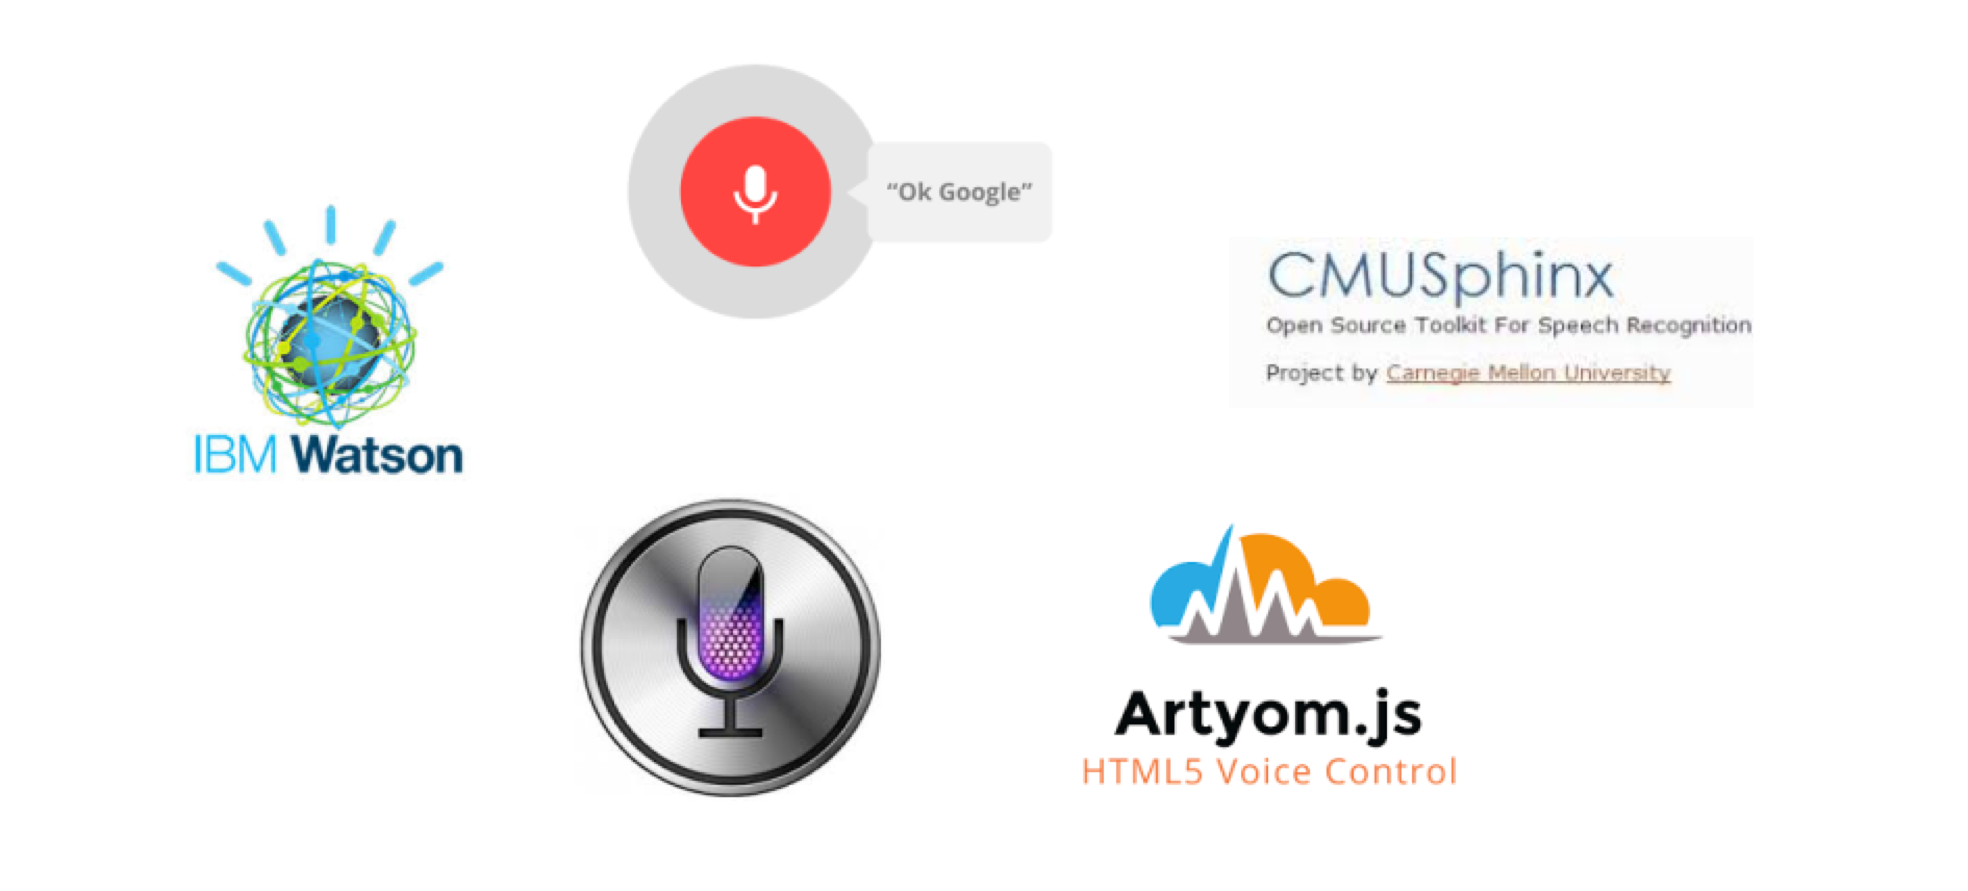
\includegraphics[width=\columnwidth]{figures/Picture2.png}.
   \caption{A few speech recognition services.}
   \label{fig:speechrecognizers}
\end{figure}
\section{Off-the-shelf speech recognition services} \mbox{} \
\label{sec:previous}

For the various solvers that we built, we used three speech recognition services - IBM Watson's Text to Speech, Wit.ai by Facebook, and Google Speech API. We call these off-the-shelf speech recognition as we did not have to build a speech recognition system using deep learning or NLP on our own to solve the audio challenges.\newline

When we started off with IBM Watson's Speech to Text API, we found that it had two accents to choose from. We also found that transcribing the same audio file using the two accents fetched us different results. In a similar case with Google's Cloud Speech API, we found we could choose from various accents in English - United States, United Kingdom, Australia and India to name a few. Thus, when we used the IBM Watson and Google Cloud Speech API solvers, we decided to explore two different accents - US and UK - and evaluated the results that we obtained by transcribing the audio with each. Wit.ai does not provide an option to specify the accent in which the audio is to be recognized. \newline

We found that both IBM Watson and Google Speech API solvers provide a list of alternative transcriptions for each recognized token in the audio. While building our response to the challenge based on the received transcription, we also looked for the tokens we wanted (like digits and alphabets) among the alternative transcription. This improved our accuracy to a great extent than just using the direct transcription received from these services. The results from these solvers were processed to convert words to digits ("one" as "1", etc.).\newline

IBM Watson service uses "machine intelligence to combine information about grammar and language structure with knowledge of the composition of an audio signal to generate an accurate transcription". It is available for free for the first 1000 min/per month for each account, after which each additional minute is charged \$ 0.02. We used multiple accounts each to access the free version of the software for the term of our project. This service can either be accessed through a WebSocket connection or through its REST API. The website provides sample code in Curl, Ruby and Node.JS with best practices for using their REST API. The API is also very well documented.\newline

